\documentclass[11pt]{article}
\usepackage[utf8]{inputenc}
\usepackage[T1]{fontenc}
\usepackage{amsmath,amssymb,amsthm}
\usepackage{graphicx,booktabs}
\usepackage[numbers]{natbib}
\usepackage{hyperref}

\newtheorem{definition}{Definition}
\newtheorem{lemma}{Lemma}

\title{CutMix in the low-data regime}
\author{A. Author \and B. Coauthor}
\date{}

\begin{document}
\maketitle

\begin{abstract}
We study CutMix when only a thousand labelled images are available. It reaches 73.2\% top-1
accuracy, most of the way to training on the full set.
\end{abstract}

\section{Introduction}

Mixing augmentations such as mixup~\cite{zhang2018mixup} and CutMix~\cite{yun2019cutmix} are standard
when data is plentiful.
Labelled images are scarce in most applied settings, and augmentations tuned on the full ImageNet
are rarely tested with a thousand images or fewer.

%%% Definition: CutMix %%%
\begin{definition}[CutMix]\label{def:cutmix}
Given two labelled images $(x_A, y_A)$ and $(x_B, y_B)$, CutMix~\cite{yun2019cutmix} forms
$\tilde{x} = M \odot x_A + (1 - M) \odot x_B$ and $\tilde{y} = \lambda y_A + (1 - \lambda) y_B$,
where $M$ is a binary box mask and $\lambda$ is the fraction of $x_A$ that it keeps.
\end{definition}
%%% end %%%

\section{Method}

%%% Definition: CutMix %%%
Recall that CutMix pastes a box of one image onto another and mixes the two labels in
proportion to the area that each image keeps.
%%% end %%%

%%% Method: Training setup %%%
We train a ResNet-50 for 200 epochs with SGD, a cosine schedule and a batch size of 256. CutMix is
applied to every batch with $\lambda \sim \mathrm{Beta}(1, 1)$.
%%% end %%%
All numbers are averaged over 5 seeds.

%%% Figure: Training loss %%%
\begin{figure}[t]
  \centering
  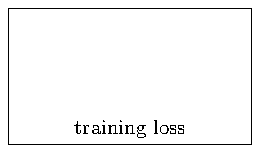
\includegraphics[width=.8\linewidth]{figures/loss.pdf}
  \caption{Training loss}\label{fig:training-loss}
\end{figure}
%%% end %%%

%%% Lemma: Mixing bound %%%
\begin{lemma}[Mixing bound]\label{lem:mixing-bound}
The mixed label $\tilde{y}$ lies in the convex hull of $y_A$ and $y_B$.
\end{lemma}
%%% end %%%


\section{Results}

%%% Result: CutMix at 1k images %%%
\paragraph{CutMix at 1k images.}
With 1k labelled images, CutMix reaches 73.2\% top-1 accuracy, against 81.4\% when trained on the
full set.
%%% end %%%

\section{Discussion}

We only looked at ResNet-50 on ImageNet subsets, so these findings may not transfer to other
backbones; a co-author rewrote this paragraph in Overleaf.

\bibliographystyle{plainnat}
\bibliography{refs}
\end{document}
